\section{Mathematics Excursion IV: Variational Calculus}

This lecture is a prelude to the following lectures that will be focused on the Lagrangian approach to mechanics, an approach that is not only equally valid but also sometimes more convenient in some scenarios to describe a system that produces the same results with perhaps some different insights. To really get into the subject, we have to introduce a little bit of additional mathematics that is necessary to understand the Lagrangian method. 

\subsection{The Euler-Lagrange Equation}
The calculus of variations is interested mostly in objects called functionals $F$, where $F: f \rightarrow \RR$ mapping functions to reals. We will be especially interested in functionals $F[y]$ of the form
\[
	F[y] = \int_{x_1}^{x_2} f(x, y, y') \, dx 
\]
for some choice of the inside function $f$. We will often look to extremize the value of this functional by an appropriate choice of a function $y$ such that $F[f]$ is a stationary point, implying that this function maximizes or minimizes the functional, but it could also be a saddle point. We don't have a good intuition for what it means for a functional to have a stationary point at a function, so we'd like to parameterize this in terms of a scalar that we can actually do regular calculus on. 

Suppose our function $y$ produces a stationary value of $F[y]$. For any small $0 \leq \epsilon \ll 1$ and a differentiable non-zero function $\xi$ such that $\xi(x_1) = \xi(x_2) = 0$, we can consider the functional $F[y + \epsilon \xi]$. Notice that we could effectively interpret this as fixing $\xi$ and making the functional solely as a function of $\epsilon$, defining 
\[
	\tilde{F}(\epsilon) = F[y + \epsilon \xi] = F[q]
\]
and letting $q = y + \epsilon \xi$ for brevity. Notice that at $\epsilon = 0$, we have $\tilde{F}(\epsilon) = F[y]$, so $\epsilon = 0$ is a stationary point of $\tilde{F}$.  

It would be nice for us to figure out a relation involving $y$ to our choice of $f$ to find the stationary points of $F[y]$. We can consider expanding $\dv{\tilde{F}}{\epsilon}$ by moving the derivative inside the integral and applying the chain rule. We will find that the term $\dv{x}{\epsilon} = 0$, since $x$ is simply the dummy variable of integration, and the terms $\dv{q}{\epsilon}$ and $\dv{q'}{\epsilon}$ will be $\xi$ and $\xi'$ by our definition of $q$. When we compute this derivative, we will get 
\begin{align*}
\dv{\tilde{F}}{\epsilon} &= \dv{}{\epsilon} \int_{x_1}^{x_2} f(x, y + \epsilon \xi, y' + \epsilon \xi') \, dx \\
&= \int_{x_1}^{x_2} \left(\pdv{f}{x} \dv{x}{\epsilon} + \pdv{f}{q} \dv{q}{\epsilon} + \pdv{f}{q'} \dv{q'}{\epsilon} \right) \, dx \\
&= \int_{x_1}^{x_2} \left(\pdv{f}{q}\xi + \pdv{f}{q'} \xi' \right) \, dx.
\end{align*}
We now "integrate by parts", by using the product rule in reverse: 
\begin{align*}
	&= \int_{x_1}^{x_2} \left(\pdv{f}{q}\xi + \dv{}{x}\left(\pdv{f}{q'}\xi \right) - \xi \dv{}{x} \pdv{f}{q'}\right) \, dx  
\end{align*}
At $\epsilon = 0$, we have $\dv{\tilde{F}}{\epsilon} = 0$, so we now plug in $\epsilon = 0$ to obtain
\begin{align*}
	0 &= \int_{x_1}^{x_2} \xi\left(\pdv{f}{y} - \dv{}{x} \pdv{f}{y'}\right) \, dx + \pdv{f}{y'}\xi \Big|_{x_1}^{x_2} \\
	&= \int_{x_1}^{x_2} \xi\left(\pdv{f}{y} - \dv{}{x} \pdv{f}{y'}\right) \, dx 
\end{align*}
where the last term vanishes because of our boundary conditions. 

We will now use the \textbf{fundamental lemma of the calculus of variations}, which states that if for continuous functions $g$ and $h$ on an open interval $(a, b)$ such that $h \neq 0$ and $h$ vanishes everywhere outside $(a,b)$, we have
\[
	\int_a^b g(x)h(x) \, dx = 0
\]
then $g(x) = 0$. 

Applying this gives the expression in parentheses is zero, so that
\[
	\pdv{f}{y} - \dv{}{x} \pdv{f}{y'} = 0.
\]
This is the \textbf{Euler-Lagrange equation}, called Euler's differential equation in the mathematical literature, and we will be seeing it frequently when discussing Lagrangian mechanics. This relation \textit{must} be true if $y$ extremizes the functional $F[y]$. 

This generalizes to if we have multiple independent variables dependent on $x$, in which case we can apply the same analysis to each of these individual variables. That being said, we then essentially require the Euler-Lagrange equation to hold true for every single one of those independent variables, independently of one another. 

Another useful equation that captures the same information as the Euler-Lagrange Equation is Euler's integral equation, which essentially combines this with the chain rule on $f$:
\[
	\dv{f}{x} = \pdv{f}{x} + \pdv{f}{y}\dv{y}{x} + \pdv{f}{y'}\dv{y'}{x}
\]
Notice also that 
\[
	\dv{}{x}\left(y' \pdv{f}{y'} \right) = \pdv{f}{y'} \dv{y'}{x} + y' \dv{}{x} \pdv{f}{y'} 
\]
and with a bit of substitution we have 
\[
	\dv{}{x}\left(y' \pdv{f}{y'} \right) = \dv{f}{x} - \pdv{f}{x} - \pdv{f}{y}\dv{y}{x} + y' \dv{}{x} \pdv{f}{y'} = \dv{f}{x} - \pdv{f}{x} + y'\left(\dv{}{x} \pdv{f}{y'} - \pdv{f}{y}\right)
\]
By Euler-Lagrange, the last term vanishes, and if $y$ has no explicit dependence on $x$, we obtain that 
\[
	\dv{}{x} \left( f - y' \pdv{f}{y'} \right) = 0
\]
or, Euler's integral equation that states 
\[
	 f - y' \pdv{f}{y'} = C
\]
for some arbitrary constant $C$.

\subsection{Constraints}
Introducing constraints into the system fixes relationships between our independent variables, which makes them correlated in some way. That is very sad, because then our previous argument of having all of the Euler-Lagrange equations for all the variables be satisfied simultaneously is on weak ground, since we argued all the variables had to be independent. Constraints also can be extremely sad, depending on what we say about the system - if the constraint can be described using an algebraic equation, then we are a bit happier and we call this constraint \textit{holonomic}. If not, obviously, we call them non-holonomic and we continue to be very sad. For example, if we confine a particle to a sphere or a surface of a ball, this is holonomic as it is described by $x^2 + y^2 + z^2 = R^2$, where $R$ is the radius of the ball - if we say instead that a particle can move around inside the ball, this is non-holonomic as now $x^2 + y^2 + z^2 \leq R^2$. Of course, these constraints  can be regular algebraic expressions, or they can be differential equations or integral expressions that must also be satisfied. Other words you might hear describing the nature of constraints: if a constraint is time-dependent, it is called \textit{rheonomic}, in contrast to being \textit{scleronomic} if it is not. 

Constraints can be dealt with in many different ways. The physical way to do it is to introduce \textit{generalized coordinates} - that is, bake the constraints into the independent coordinates you are using for the system. For example, if we have a constraint normal force on a system, we can choose a coordinate perpendicular to the normal force so that it does no work, thus eliminating that constraint explicitly. 

%Another way to do this is with the Lagrange multipliers method, which works by considering \textit{variations} of the functional $F$ when $F$ is stationary, and tacks on the constraints. When extremized, if $F$ is displaced virtually by $\delta F$, we can express this variation in terms of virtual displacements of the $n$ coordinates: 
%\[
%	\delta F = \sum_i^n \pdv{F}{q_i} \delta q_i
%\]
%If we also have $m$ holonomic constraints, when $F$ is varied, we 
\subsection{Examples} 
\subsubsection{The Path With The Shortest Distance Between Two Points Is...}
\begin{problem}
Suppose we have two points, labeled $1$ and $2$, on a Cartesian plane. Find the path that minimizes the distance between these two points. 
\end{problem}

\begin{solution}
We will do this variationally. Let $y$ be the desired minimal path. Note that the infinitesimal arc length of the path, $ds$, is given by $\sqrt{dx^2 + dy^2} = \sqrt{1 + \left(\dv{y}{x}\right)^2} \, dx$, so it suffices to minimize the integral functional
\[
	L = \int_1^2 \sqrt{1 + \left(\dv{y}{x}\right)^2} \, dx = \int_1^2 \sqrt{1 + y'^2} \, dx.
\]
Applying Euler-Lagrange, we see no explicit dependence on $y$, so we get that 
\[
	\dv{}{x} \frac{y'}{\sqrt{1+y'^2}} = 0 \implies
	\frac{y'}{\sqrt{1+y'^2}}  = C
\]
for some real $C$. Rearranging, we get 
\[
	y'^2 = a
\]
for some (other) real constant, so $\dv{y}{x}$ is a constant. That means that $y$ must be a line, as known by Euclid some millenia ago. 
\end{solution}

\subsubsection{The Brachistocrone Problem}
\begin{problem}
Find the shape of the path that minimizes the transit time between two points at different elevations under the influence of a uniform gravitational field.
\end{problem}

\begin{solution}
Let us set our potential to be zero at the top of our path, where we also set $y = 0$. By conservation of energy, we have the velocity at any given elevation to be $v = \sqrt{2gy}$. Thus, the total transit time $T$ is computed by integrating over the entire length of the path: 
\[
	T = \int_1^2 \frac{ds}{v} = \int_1^2 \sqrt{\frac{dx^2 + dy^2}{2gy}} = \int_1^2 \sqrt{\frac{x'^2  + 1}{2gy}} \, dy 
\]
Since the constant $\frac{1}{\sqrt{2g}}$ just comes out of the integral, we are only concerned with using Euler-Lagrange on $f(x, y) = \sqrt{\frac{x'^2  + 1}{y}}$. Notice that $\pdv{f}{x} = 0$, so we can integrate to get
\[
	\frac{x'}{\sqrt{y(1 + x'^2)}} = C
\]
for some constant $C$. With some foresight and rearrangement, we can replace the constants enough so that we get 
\[
	x' = \frac{y}{\sqrt{2ay-y^2}}
\]
To integrate this, we consider the substitution $y = a(1-\cos\theta)$, which yields a lot of cancellations and gives $x = a(\theta - \sin \theta)$. This result can be interpreted as the curve traced when a circle rolls across a flat surface, which is called a \textit{cycloid}. For reference, a sketch of the curve is given below: 
\begin{center}
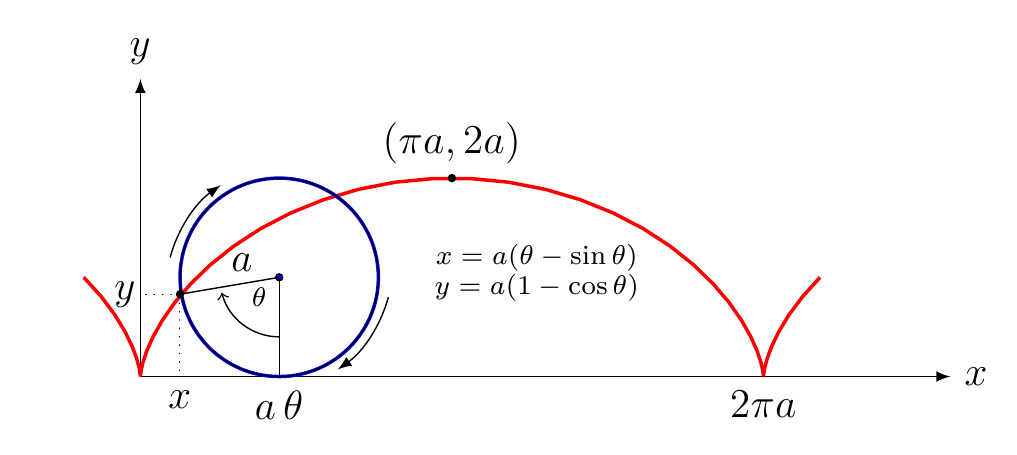
\includegraphics[scale=0.3]{images/mechadv/cycloid.png}
\end{center}

\end{solution}

\subsection{Exercises}
\begin{enumerate}
\item Find and describe the path $y = y(x)$ for which the integral 
\[
	\int_{x_1}^{x_2} \sqrt{x} \sqrt{1 + y'^2} \, dx 
\]
is stationary. 

\item This problem concerns the \textit{catenary}, a shape formed when a uniform rope of fixed length hangs under the force of gravity. Show that, by minimizing the gravitational potential energy and constraining the length to be fixed, the rope takes the shape of a $\cosh$ curve, that is, a hyperbolic cosine curve. 

\item Find the minimal surface between two circles of radius $R$ with centers aligned along the $z$-axis, with a distance of $h$ between them. Choose your independent variables and coordinate systems wisely. Does the solution look familiar? 

\item This concerns the time traveled between two points on a cycloid. A cycloid is traced out by a point on a circle of radius $a$ as the circle rolls without slipping for one revolution. Suppose a mass is released from rest at any point $P_0$ associated with angle $\theta_0$, $0 < \theta_0 < \pi$, on the track between the highest point $O$ and the lowest point $P$. Compute the time it takes for the mass to reach $P$ as the integral 
\[
	\sqrt{\frac{a}{g}} \int_{\theta_0}^\pi \sqrt{\frac{1-\cos\theta}{\cos\theta_0 - \cos \theta}} \, d\theta 
\]
and evaluate this integral as $\pi \sqrt{\frac{a}{g}}$.

\item Find the dimensions of the parallelopiped of maximum volume circumscribed by a sphere of radius $R$. 


\end{enumerate}